\section{Discrete random probability measures}


\subsection{Introduction}


\begin{frame}{References}
\begin{itemize}
	\item \alert{One of the first textbooks on the Dirichlet process}: \fullcite{Ghosh2003}
	\item \alert{One that reads very well}: \fullcite{hjort2010bayesian}
	\item \alert{Chapter 14} on Discrete Random Structures of \fullcite{ghosal2017fundamentals}
\end{itemize}
\end{frame}


\subsection{Dirichlet process}

\begin{frame}{Dirichlet distribution}
	The \textit{Dirichlet distribution} on the simplex $\Delta_K$ is a probability distribution with parameter $\boldsymbol{\alpha} = (\alpha_1,\ldots,\alpha_K)$ with $\alpha_j>0$ and density function, for $\boldsymbol{x} = (x_1, \ldots, x_K)\in \Delta_K$,
\begin{displaymath}
f(\boldsymbol{x}; \boldsymbol{\alpha}) = \frac{1}{B(\alpha)}\prod_{i=1}^Kx_i^{\alpha_i - 1}.
\end{displaymath}
% where $(x_i)$ form a simplex. 

The Dirichlet distribution is conjugate for the multinomial distribution. 

\begin{center}
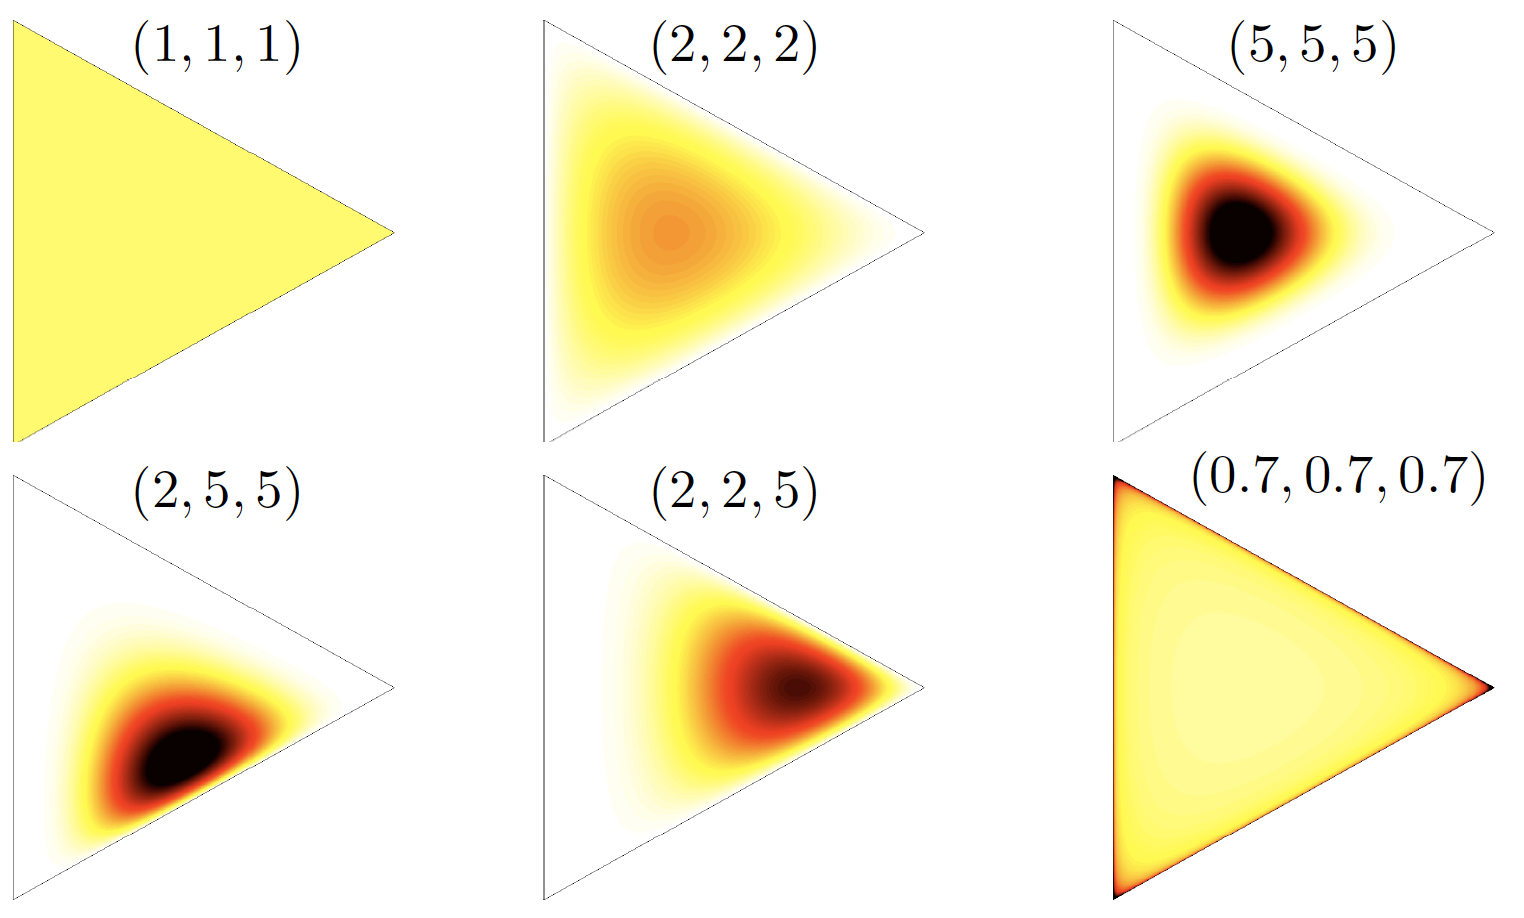
\includegraphics[width = .6\textwidth]{figures_julyan/intro_DP/dirichlet_distribution}
\end{center}
\hfill\textcolor{gray}{[Image by Y.W. Teh]}
\end{frame}


\begin{frame}{Dirichlet process}
A central Bayesian nonparametric prior \citep{ferguson1973bayesian}.\pause

\begin{block}{Definition (Dirichlet process)}
A \alert{Dirichlet process} on the space $\mathcal{Y}$ is a random process $ P $ such that there exist $ \alpha>0 $ (precision parameter) and $ P_0 $ (base/centering distribution) \pause such that for any finite partition $ \{A_1,\ldots,A_k\} $ of $\mathcal{Y}$, the random vector
$ (P(A_1),\ldots,P(A_k)) $ is Dirichlet distributed
\[ (P(A_1),\ldots,P(A_k))\sim \text{Dir}(\alpha P_0(A_1),\ldots,\alpha P_0(A_k)) \]
\textit{Notation}: $ P \sim \text{DP}(\alpha, P_0) $
\end{block}
\begin{center}
\visible<3->{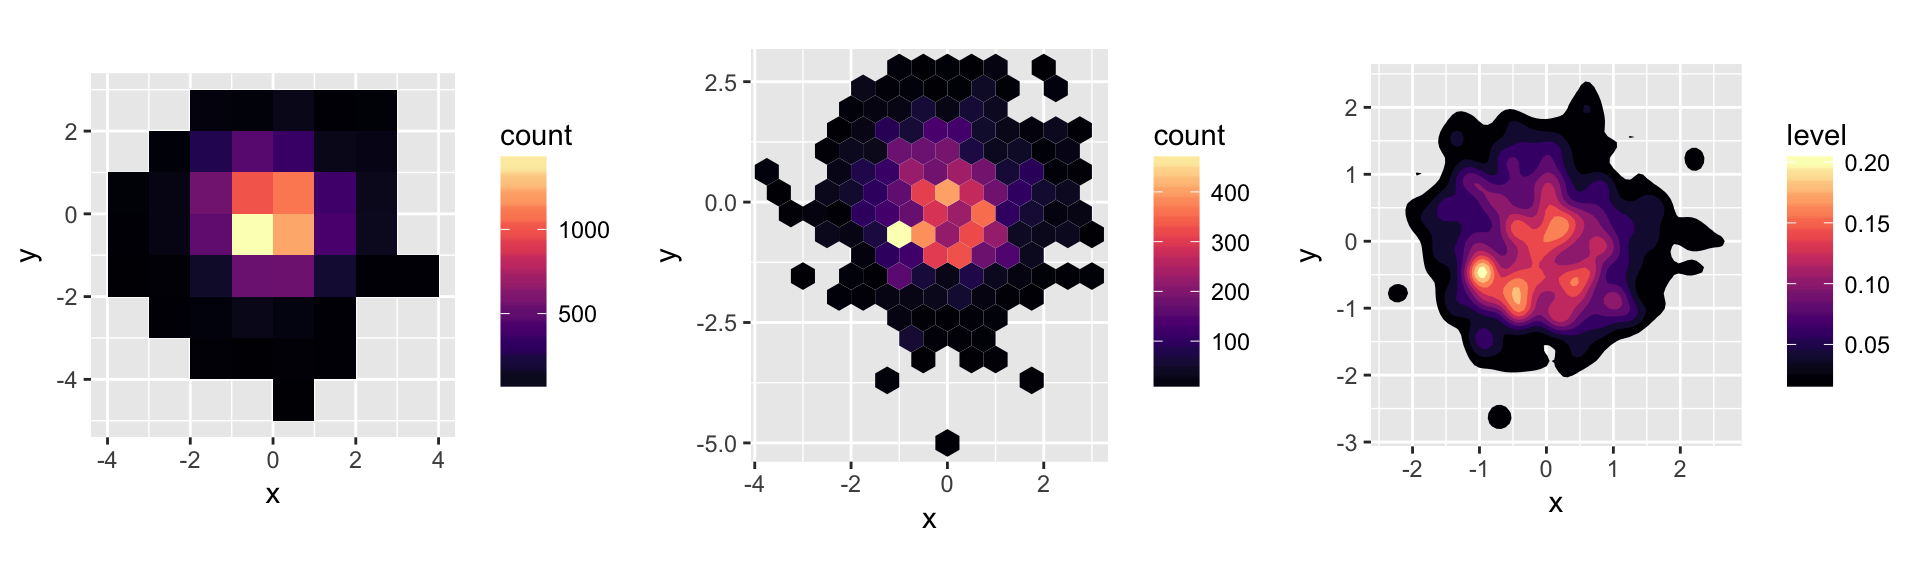
\includegraphics[width=\textwidth]{figures_julyan/intro_DP/DP_marginal}}
%\animategraphics[loop, width=\textwidth]{2}{figures_julyan/intro_DP/density_2D_}{1}{10} % pb ici: should specify pdf for images...
\end{center}
\end{frame}

\begin{frame}[allowframebreaks]{Moments of Dirichlet process}
	\begin{proposition}
Let $P\sim \text{DP}(\PrecisonParam, P_0)$ then for every measurable sets $A, B$ we have
\begin{align*}
    \E[ P(A)] &= P_0(A),\\
    \Var[P(A)] &= \frac{P_0(A)(1-P_0(A))}{1+\PrecisonParam},\\
    \Cov( P(A), P(B) )&=\frac{P_0(A \cap B) - P_0(A)P_0(B) }{1+\PrecisonParam}\label{Dir:Covariance}.
\end{align*}
\end{proposition}

% \begin{enumerate}
%     \item $\E( p(A)) = P_0(A)$,
%     \item ${\rm Var}(p(A)) = \frac{P_0(A)(1-P_0(A))}{1+\PrecisonParam}$,
%     \item $\Cov( p(A), p(B) )=\frac{P_0(A \cap B) - P_0(A)P_0(B) }{1+\PrecisonParam}$.
% \end{enumerate}
\framebreak

\textbf{Proof.}
We will make use of  $p(A)\sim \Beta(\alpha P_0(A), \alpha (1-P_0(A)))$. From this we obtain 
\begin{equation*}
    \E (p(A)) = \frac{\PrecisonParam P_0(A)}{\PrecisonParam( P_0(A) + 1 - P_0(A) )} = P_0(A)
\end{equation*}
and 
\begin{equation*}
    \Var(p(A))=\frac{\PrecisonParam^2 P_0(A)( 1-P_0(A) )}{\PrecisonParam^2 (\PrecisonParam + 1)}.
\end{equation*}
We derive the covariance term in two cases, firstly taking into consideration the one with $A\cap B = \emptyset$. In that case any space $\Omega$ may be decomposed into three sets: 
$$
\Omega = \{A, B, (A\cup B)^c\}.
$$
Using de Morgan's law the last can be written as $(A\cup B)^c = A^c\cap B^c =: C$. Therefore we may write a joint probability vector
\begin{equation*}
    \big( P(A), P(B), P(A^c\cap B^c) \big)\sim \Dir\big(\PrecisonParam P_0(A), \PrecisonParam P_0(B), \PrecisonParam P_0(C) \big)
\end{equation*}
and hence $\Cov(P(A), P(B)) = -P_0(A)P_0(B)/(1+\PrecisonParam) $. 
In the more general case one may decompose 
\begin{align*}
    A &= (A\cap B) \cup (A\cap B^c)\\
    B &= (B\cap A)\cup (B\cap A^c),
\end{align*}
so that 
\begin{equation*}
    \begin{split}
    \Cov (P(A), P(B)) &= \Cov (P(A\cap B) +P(A\cap B^c), P(B\cap A) + P(B\cap A^c) ) 
    % &=\Cov (P(A\cap B) , P(B\cap A)  ) + \Cov (P(A\cap B),  P(B\cap A^c) ) +\\
    % &+\Cov (P(A\cap B^c), P(B\cap A)  ) + \Cov (P(A\cap B^c),  P(B\cap A^c) ),
    \end{split}
\end{equation*}
and so forth using the linearity of covariance.\hfill $\square$
\end{frame}


\begin{frame}{Marginalizing out the DP}
	Property $\E[ P(A)] = P_0(A)$ can be written equivalently as
\begin{equation*}
    \E( P(A)) = P_0(A) = \int P(A)\ddr \text{DP}(P). 
\end{equation*}

%
%The precision parameter $\PrecisonParam$ in $DP(\PrecisonParam, P_0)$ controls variability of $P(A)$ around $P_0(A)$, so called \textit{base measure} of underlying Dirichlet process. 

A Dirichlet process model can be constructed as a two level sampling model:
\begin{equation*}
    \left \{ \begin{matrix}
P \sim \text{DP}(\PrecisonParam, P_0)\\ 
X|P \sim P,
\end{matrix}\right.
\end{equation*}
i.e. we  sample a probability measure $P$ from the Dirichlet process and then given  $P$, we sample random variables $X_i$.\bigskip

\textcolor{red2}{Marginalizing out $P$}, we obtain the marginal distribution of $X$:
$$X\sim P_0.$$

\end{frame}


\begin{frame}[allowframebreaks]{Posterior distribution}
	Let $X_{1:n} := (X_1,\ldots, X_n)$ be sampled from the hierarchical model 
\begin{equation*}
    \left \{ \begin{matrix}
P \sim \text{DP}(\PrecisonParam, P_0)\\ 
X_{1:n}|P \simiid P.
\end{matrix}\right.
\end{equation*}
This model is usually used as a building block in a larger hierarchical model, e.g. mixture models, graphs, etc. 
\begin{theorem}[DP posterior distribution] 
The DP is \alert{conjugate}, with posterior equal to
\begin{equation*}
    P|X_{1:n}\sim \text{DP}(\PrecisonParam P_0 + \sum_{i=1}^n\delta_{X_i}).
\end{equation*}
The \alert{predictive distribution}, called \alert{P\'olya urn} or \alert{Blackwell--MacQueen scheme}, is given by
\begin{equation*}
    \P(X_{n+1} | X_{1:n}) = \frac{\PrecisonParam}{\PrecisonParam +n} P_0 + \frac{1}{\PrecisonParam + n}\sum_{i=1}^n\delta_{X_i}.
\end{equation*}
\end{theorem}

\framebreak

\textbf{Proof.}
The posterior distribution of $\boldsymbol{a} = (a_1, \ldots, a_k) = ( P(A_1), \ldots, P(A_k) )$ depends on the observations only via their cell counts $\boldsymbol{N}= (N_1, \ldots, N_k)$, $N_j = \# \{ i : X_i \in A_j\}$  (it comes from \textit{tail--free} property), so
\begin{equation*}
  \boldsymbol{a} \vert X_{1:n}\sim \boldsymbol{a} \vert N_{1:k}.
\end{equation*}
The prior  and model are
\begin{equation*}
    \left \{ 
    \begin{matrix}
\boldsymbol{a} \sim \Dir_k (\PrecisonParam P_0(A_1), \ldots, \PrecisonParam P_0(A_k))
\\
\boldsymbol{N}\vert P \sim {\rm Multinom}_k (\boldsymbol{a}).
\end{matrix}\right.
\end{equation*}
This results in the posterior of form 
\begin{align*}
    p(\boldsymbol{a}\vert \boldsymbol{N}) 
    &\propto a_1^{\PrecisonParam P_0(A_1) +N_1-1}\cdots a_k^{\PrecisonParam P_0(A_k)+N_k -1}\\ 
    &= \Dir_k\big( \PrecisonParam P_0(A_1) +N_1, \ldots, \PrecisonParam P_0(A_k) +N_k\big).
\end{align*} \hfill $\square$
%Property (\ref{Dir:predictive}) is a result of taking the expected value of (\ref{Dir:posterior}). \hfill $\square$
\end{frame}


%----------------
% Combinatorial properties: Number of distinct values
\begin{frame}[allowframebreaks]{Combinatorial properties: Number of distinct values}

Assume that the base measure $P_0$ is non-atomic. Then  with probability 1:
$$
X_i\notin\{X_1,\ldots, X_{i-1}\} \Leftrightarrow X_i \sim P_0.
$$
% what means that $X_i$ is a new value.
Let $D_i =  \mathbb{I}(X_i \text{ is a new value})$ and lets denote $K_n=\sum_{i=1}^nD_i$, a number of distinct values $X_1,\ldots, X_n$ with distribution $\mathcal{L}(K_n)$.
\begin{proposition}[Asymptotics for $K_n$]
Random variables $D_i$ are distributed i.i.d. with respect to $Bernoulli(\PrecisonParam/(\PrecisonParam + i - 1))$. Therefore for fixed $\PrecisonParam$ and for $n\rightarrow \infty$ we have:
\begin{enumerate}
    \item[i)] $\E K_n\sim \PrecisonParam \log n \sim \Var(K_n)$
    \item[ii)] $K_n/\log(n)\xrightarrow{a.s.} \PrecisonParam$
    \item[iii)] $(K_n - \E K_n)/\text{sd}(K_n)\rightarrow N(0,1) $
    \item[iv)] $\text{d}_{\text{TV}}\big( \mathcal{L}(K_n), \text{Poisson}(\E K_n) \big)=o \big(1 / \log(n)\big)$ where $$
    \text{d}_{\text{TV}}(P,Q)=\text{sup}|P(A)-Q(A)|
    $$
    over measurable  partition $A$
\end{enumerate}
\end{proposition}

\framebreak

\textbf{Proof.}
\begin{enumerate}
    \item[i)] $\E K_n = \sum_{i=1}^n \frac{\PrecisonParam}{\PrecisonParam+i-1} $ and $ \Var(K_n) = \sum_{i=1}^n\frac{\PrecisonParam(i-1)}{(\PrecisonParam + i -1)^2}$.
    \item[ii)] Since $D_i$'s are $\mathbb{I}$ one may use Kolmogorov law of strong numbers and 
    $$
    \sum_{i=1}^\infty \frac{\Var (D_i)}{ (\log i)^2 }= \sum_{i=1}^\infty \frac{\PrecisonParam(i-1)}{(\PrecisonParam +i-1)^2 (\log i)^2}<\infty$$
    by e.g. the fact that $\sum_i (1/i(\log i)^2)$ converges.
    \item[iii)]By Lindeberg central limit theorem.
    \item[iv)] This is implied from Chein--Stein approximation. %https://faculty.math.illinois.edu/~psdey/414CourseNotes.pdf 
\end{enumerate}
\hfill $\square$
\framebreak

A central limit theorem for independent random variables (possibly not identically distributed).

\begin{theorem}[Lindeberg central limit theorem]
Suppose $X_i$ are i.i.d. such that $\E X_i = \mu_i$ and $\Var X_i = \sigma_i^2 <\infty$. Define $Y_i = X_i - \mu_i,\ T_n = \sum_{i=1}^n Y_i,\ s_n^2 = \Var (T_n) = \sum_{i=1}^n\sigma_i^2$. Then provided that
\begin{equation*}
    \forall \epsilon > 0\quad \frac{1}{s_n^2}\sum_{i=1}^n\E \big(Y_i^2 \mathbb{I}(|Y_i|>\epsilon s_n) \big)\xrightarrow{n\rightarrow \infty} 0 \text{[Lindeberg condition],}
\end{equation*}
we have the central limit theorem: $T_n/s_n \xrightarrow{\small{d}}N(0,1)$.
\end{theorem}

\end{frame}



%------------
% Combinatorial properties: Distribution of distinct values
\begin{frame}[allowframebreaks]{Combinatorial properties: Distribution of distinct values}
	We have now the limits of $K_n$ and we know its approximate distribution $\mathcal{L}(K_n)$. The \alert{exact distribution of $K_n$} is:
\begin{proposition}[Distribution of $K_n$]
If $P_0$ is non-atomic then 
\begin{equation}\label{distr_of_Kn}
    \P(K_n=k) = \mathfrak{C}_n(k) n!\PrecisonParam ^k \frac{\Gamma(\PrecisonParam)}{\Gamma(\PrecisonParam+n)},
\end{equation}
where 
\begin{equation}\label{mathfrakC_def}
\mathfrak{C}_n(k)=\frac{1}{n!}\sum_{S\in\mathfrak{J}_n(k)} \prod_{j\in S}j    
\end{equation}
and $\mathfrak{J}_n(k)=\{ S\subset \{ 1,\ldots,n-1\},\ |S|=n-k \}$.
\end{proposition}

 Recall the definition of the \alert{Gamma function} $\Gamma(x)=\int_0^\infty u^{x-1}e^{-u}du$.
 
\framebreak



Let us consider when we may deal with events $K_n = k$: we have two cases
\begin{equation*}
    \left \{ \begin{matrix}
K_{n-1}=k-1 \text{ and } X_n \text{ is a new value}\\
K_{n-1} = k \text{ and } X_n \text{ is not a new value}.
\end{matrix}\right.
\end{equation*}
 This results in
% either in proceeding case $K_{n-1}$ we have $K_{n-1}=k-1 $ and $X_n$ is a new value or we have $K_{n-1} = k$ and $X_n$ does not take new value.
\begin{equation}\label{CombinatorialProperties}
    p_n(k,\PrecisonParam) := \P(k_n = k|\PrecisonParam) = \frac{\PrecisonParam}{\PrecisonParam +n -1 }p_{n-1} (k-1,\PrecisonParam)+\frac{n-1}{\PrecisonParam +n -1}p_{n-1}(k,\PrecisonParam).
\end{equation}
Now let us remark that $\mathfrak{C}_n(k)=p_n(k,\PrecisonParam =1)$. Therefore
\begin{equation}\label{mathfrakC_property}
    \mathfrak{C}_n(k)=\frac 1n \mathfrak{C}_{n-1}(k-1)+\frac{n-1}{n}\mathfrak{C}_{n-1}(k).
\end{equation}
By induction over $n$: first we check case $n=1$:
\begin{equation*}
    p_1(1,\PrecisonParam)=\mathfrak{C}_1(1)\frac{\PrecisonParam}{\PrecisonParam}=\mathfrak{C}_1(1).
\end{equation*}
To check case $n>1$ we use (\ref{distr_of_Kn}) and then (\ref{CombinatorialProperties}):
\begin{equation*}
    \begin{split}
        p_n(k,\PrecisonParam)&=\frac{\PrecisonParam}{\PrecisonParam +n -1 }p_{n-1} (k-1,\PrecisonParam)+\frac{n-1}{\PrecisonParam +n -1}p_{n-1}(k,\PrecisonParam) \\
        &=\frac{\PrecisonParam}{\PrecisonParam +n -1 }\mathfrak{C}_{n-1}(k-1)(n-1)!\PrecisonParam^{k-1}\frac{\Gamma (\PrecisonParam)}{\Gamma(\PrecisonParam+n-1)} +\\
        &+\frac{n-1}{\PrecisonParam +n -1}\mathfrak{C}_{n-1}(k)(n-1)!\PrecisonParam^{k}\frac{\Gamma (\PrecisonParam)}{\Gamma(\PrecisonParam+n-1)}\\
        &=\frac{\PrecisonParam^k}{\PrecisonParam+n-1}(n-1)!\frac{\Gamma(\PrecisonParam)}{ \Gamma(\PrecisonParam+n-1) }n\bigg(\frac 1n \mathfrak{C}_{n-1}(k-1) + \frac{n-1}{n} \mathfrak{C}_{n-1}(k)\bigg)\\
        &=\mathfrak{C}_{n}(k)n!\PrecisonParam^k\frac{\Gamma(\PrecisonParam)}{\Gamma(\PrecisonParam+n)},
    \end{split}
\end{equation*}
which proves property (\ref{distr_of_Kn}).

To prove (\ref{mathfrakC_def}) let use define a polynomial $A_n(s)$ as $A_n(s) = \sum_{i=1}^\infty \mathfrak{C}_n(k)s^k$. Then using (\ref{mathfrakC_property}) polynomial $A_n(s)$ can be written as
\begin{equation*}
\begin{split}
    A_n(s)&=\sum_{k=1}^\infty \bigg(  \frac 1n \mathfrak{C}_{n-1}(k-1)+\frac{n-1}{n}\mathfrak{C}_{n-1}(k)   \bigg) s_k\\
    &=\frac{1}{n}( s A_{n-1}(s) +(n-1) A_{n-1}(s) )=\frac{s+n-1}{n}A_{n-1}(s)\\
    &=\ldots=A_1(s)\prod_{j=2}^n\frac{s+j-1}{j}=\frac{s(s+1)\cdot\ldots\cdot(s+n-1)}{n!}.
\end{split}
\end{equation*}
Last equality implies from the fact that $\mathfrak{C}_1(k)=\ind\{k=1\}$ and hence $A_1(s)=s$. Checking terms after the expansion finishes the proof of (\ref{mathfrakC_def}).


\end{frame}




%------------
% Combinatorial properties: CRP
\begin{frame}[allowframebreaks]{Combinatorial properties: Chinese Restaurant process}
A culinary metaphor of the \alert{random partition} induced by the DP. Customers join tables with probability proportional to \alert{$n_j$}, the number of clients already sitting, or sit at new table with probability  proportional to \alert{$\PrecisonParam$}.
\begin{center}
	\includegraphics[width = .5\textwidth]{figures_julyan/intro_DP/CRP}
\end{center}

\begin{proposition}[Chinese Restaurant process]
A random sample $X_{1:n}$ from a DP with precision parameter $\PrecisonParam$ induces a partition of $\{1,\ldots,n\}$ into $k$ sets of sizes $n_1,\ldots,n_k$ with probability 
\begin{equation*}
    p(n_1,\ldots,n_k)=p(\{n_1,\ldots,n_k\})=\PrecisonParam^k\frac{\Gamma(\PrecisonParam)}{\Gamma(\PrecisonParam+n)}\prod_{j=1}^k\Gamma (n_j).
\end{equation*}
\end{proposition}

\framebreak
\textbf{Proof.}
	We use the P\'olya urn scheme slightly changed by using $n_1,\ldots, n_k$
\begin{equation*}
    \P(X_{n+1}|X_{1:n})=\frac{\PrecisonParam}{\PrecisonParam + n}P_0 + \frac{1}{\PrecisonParam + n}\sum_{j=1}^kn_j\delta_{X^*_j}.
\end{equation*}
    By exchangeability, the distribution of $\{n_1,\ldots, n_k\}$ does not depend on the order of the observations. Let's compute $p(n_1,\ldots, p_k)$ as the probability of one draw where the first table consists of first $n_1$ observations etc. 
    
    To proceed, let us use P\'olya urn scheme: we denote $\bar{n}_j=\sum_{i=1}^jn_i$ and hence $\bar{n}_k=n$, the total number of observations. We can observe the following pattern: first ball open new table, following $n_j-1$ ones fill in that table and so forth. That quantity can be rewritten as 
    $$
    \frac{\PrecisonParam^k}{\PrecisonParam(\PrecisonParam+1)\ldots(\PrecisonParam+n-1)}\prod_{j=1}^k(n_j-1)!,
    $$
where one can rewrite both terms using Gamma function $\Gamma(x)=\int_0^\infty u^{x-1}e^{-u}du$: the first  term  can be written as 
$$
\frac{\PrecisonParam^k}{\PrecisonParam(\PrecisonParam+1)\ldots(\PrecisonParam+n-1)}=\frac{\Gamma(\PrecisonParam+n)}{\Gamma(\PrecisonParam)},
$$
while the second one as
$(n_j-1)!=\Gamma(n_j)$.

One should remark that for ordered partitions we have 
$$
\bar{p}(n_1,\ldots,n_k)=\frac{p(n_1,\ldots,n_k)}{k!}.
$$
\hfill $\square$
\end{frame}


%
%%------------
%% Combinatorial properties: Ewens
%\begin{frame}[allowframebreaks]{Combinatorial properties: Ewens sampling formula}
%\end{frame}
%
%



%------------
% Combinatorial properties: Ewens
\begin{frame}[allowframebreaks]{Combinatorial properties: Ewens sampling formula}

Ewens sampling formula (ESF), presented originally by \citet{ewens1972sampling}, is the distribution of multiplicities $m=(m_1,\ldots, m_n)$, $m_\ell$ is the number of groups of size $\ell$.
Also known as allelic partitions in population genetics, when there is no selective difference between types: null hypothesis in non Darwinian theory.
See also \citet{antoniak1974mixtures}.

\begin{proposition}[Ewens sampling formula]\label{ESF}
The distribution of the multiplicities $(m_1,\ldots, m_n)$ induced by a DP is
\begin{equation*}
    p(m_1,\ldots, m_n)=\frac{\PrecisonParam^k}{\PrecisonParam_{(n)}}\frac{n!}{\prod_{\ell=1}^n \ell^{m_\ell}m_\ell!}.
\end{equation*}
\end{proposition}\bigskip

Notation $n_{(k)}:=n(n-1)\cdots(n-k+1)$.



%\vskip -1cm
%\begin{center}
%	\includegraphics[width = .6\textwidth]{figures_julyan/CRP}
%\end{center}

\framebreak
\textbf{Proof.}
Two steps: 1) Compute probability of particular sequence of $X_1, \ldots, X_n$ in given class $(m_1,\ldots,m_n)$, note that all such sequences are equally likely and 2) multiply obtained quantity by the number of such sequences. 

\begin{itemize}
    \item[1)] Consider a sequence $X_1,\ldots, X_n$ such that $X_1, \ldots, X_{m_1}$ occur each only once, then the next $m_2$ occur only twice and so on. This sequence has probability which may be obtained by the P\'olya Urn scheme in the same fashion as CRP:
    \begin{equation*}
        \frac{\PrecisonParam^{m_1} (\PrecisonParam \cdot 1)^{m_2} \ldots \big( \PrecisonParam \cdot 1 \cdot\ldots \cdot (n-1) \big)^{m_n}  }{\PrecisonParam_{(n)}}=\frac{\PrecisonParam^k}{\PrecisonParam_{(n)}}\prod_{\ell=1}^n ((\ell-1)!)^{m_\ell}.
    \end{equation*}
%    Each term in the numerator comes from $m_\ell$ species observed $\ell$ times.
    \item[2)] Number of sequences $X_1,\ldots,X_n$ with frequencies $(m_1, \ldots, m_n)$ is a number of ways of putting $n$ distinct objects into bins, so called multinomial coefficient. Since ordering of the $m_\ell$ bins of frequency $\ell$ is irrelevant,  divide by $m_\ell!$:
    \begin{equation*}
        \frac{1}{\prod_{l=1}^n (m_\ell)!}
        \begin{pmatrix}
n\\ 
1\times \# m_1, 2\times \# m_2, \ldots, n\times \# m_n
\end{pmatrix}
= \frac{n!}{\prod_{\ell=1}^n m_\ell!(\ell!)^{m_\ell}}
    \end{equation*}
\end{itemize}
To finish one needs to multiply results obtained in 1) and 2). \hfill $\square$
\end{frame}




%-------------
% Stick-breaking

\begin{frame}{Stick-breaking representation}
The \alert{DP} has almost surely \alert{discrete} realizations (Sethuraman, 1994)\pause

\begin{minipage}{.55\textwidth}
$$P=\sum_{j=1}^{\infty}\pi_{j}\delta_{\theta_{j}}\,\text{ }$$
\begin{itemize}
\item locations $\theta_{j}\simiid G_{0}$ %(Sethuraman 1994)%\citp{se}
\item %weights $p_{j}$ defined by 
weights $\pi_{j}=\tilde \pi_j\prod_{l<j}(1-\tilde \pi_{l})$ with $\tilde \pi_{j}\simiid Beta(1,\alpha)$,\pause
\end{itemize}\medskip
\visible<4->{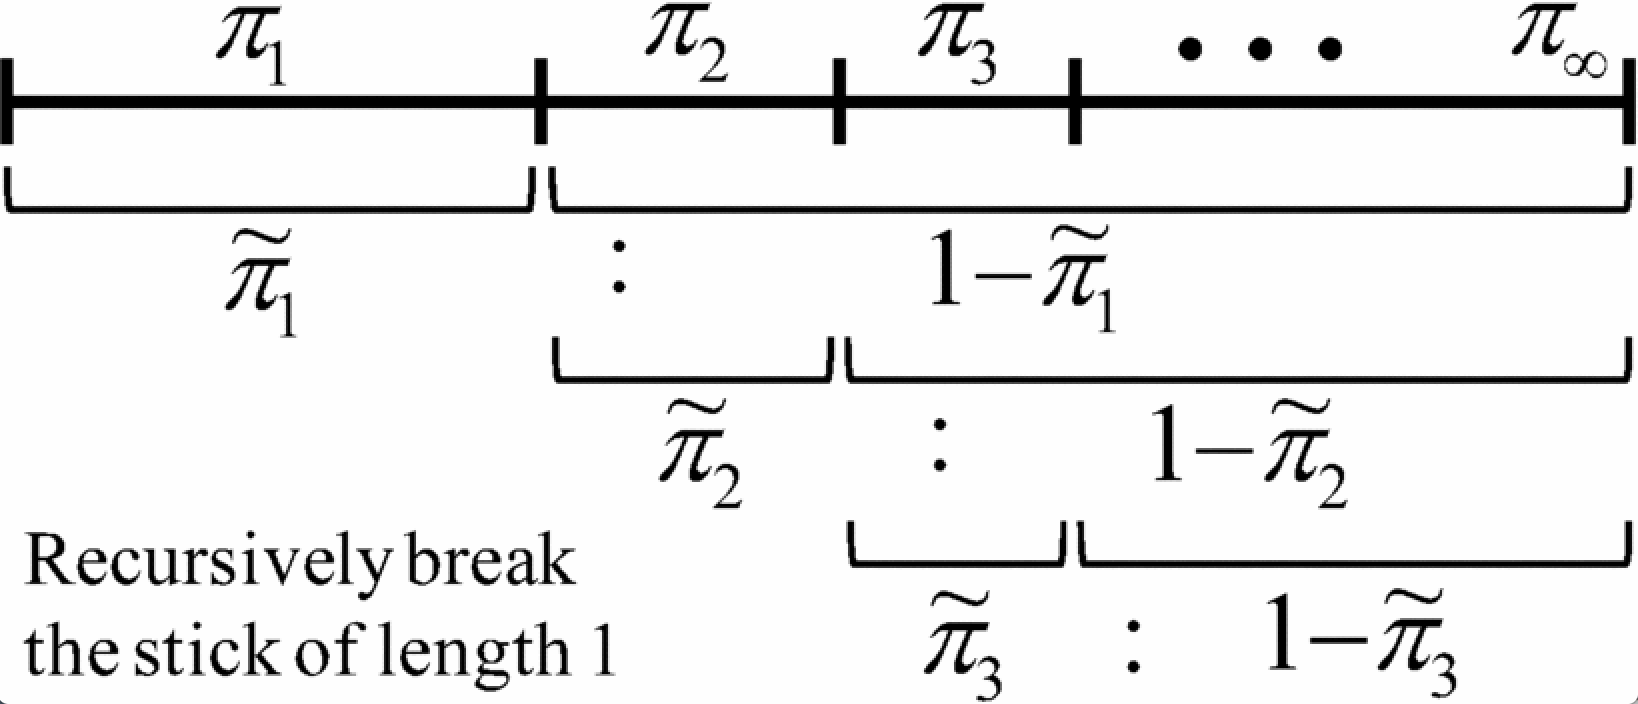
\includegraphics[width=\textwidth]{figures_julyan/intro_DP/sb}}
\end{minipage}\hskip.5cm
\begin{minipage}{.4\textwidth}
\visible<5->{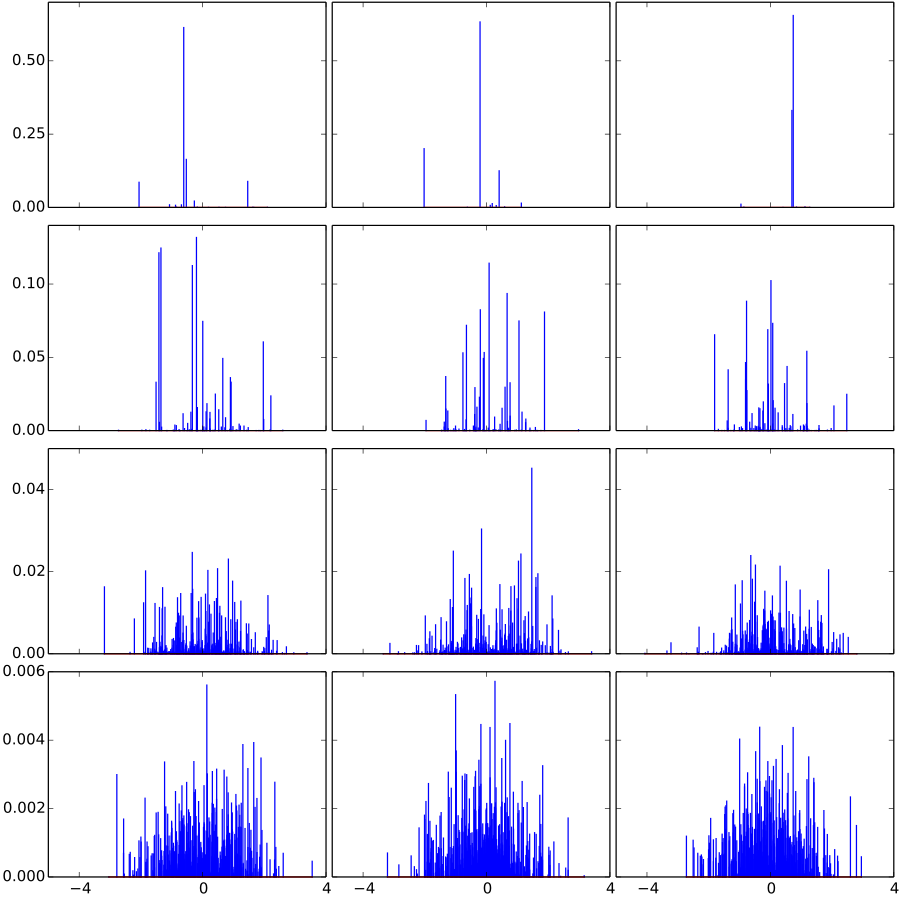
\includegraphics[width=\textwidth]{figures_julyan/intro_DP/DP}}
%\visible<5->{\includegraphics[width=\textwidth]{figures_julyan/intro_DP/SB-1}}
%\visible<6->{\includegraphics[width=\textwidth]{figures_julyan/intro_DP/SB-2}}
%\visible<7->{\includegraphics[width=\textwidth]{figures_julyan/intro_DP/SB-3}}
%\visible<8->{\includegraphics[width=\textwidth]{figures_julyan/intro_DP/SB-4}}
\end{minipage}
%($\delta_{\theta_{j}}$ stands for the Dirac mass at point $\theta_{j}$)

\end{frame}

\begin{frame}[allowframebreaks]{Stick-breaking representation}

A constructive representation of the DP due to \citet{sethuraman1994constructive}.
\begin{theorem}[Stick-breaking]\label{theorem:sethuraman}
If $V_1, V_2, \ldots \simiid Be(1, \PrecisonParam)$ and $\phi_1, \phi_2, \ldots \simiid P_0$ are i.i.d. variables, then define $p_1=V_1$ and 

$$
p_j=V_j \prod_{1\leq l \leq j}(1-V_l)
$$ 
then 
$$
P=\sum_{i=1}^\infty p_i\delta_{\phi_i}\sim \text{DP}(\PrecisonParam, P_0).
$$
\end{theorem}

\pause

\begin{lemma}
For independent $\phi\sim P_0$ and $V\sim Be(1,\PrecisonParam)$ the DP is the only solution of the distributional equation 
\begin{equation*}\label{Dir:distributional_equation}
    P \sim V\delta_\phi + (1-V)P, 
\end{equation*}
where $P\sim \text{DP}(\PrecisonParam, P_0)$.
\end{lemma}

%We say that such a RPM is solution of (\ref{Dir:distributional_equation}) if $P$ is independent of $(V, \phi)$ and if for every measurable partition $(A_1, \ldots, A_k)$ of $X$ both sides of (\ref{Dir:distributional_equation}) are random vectors equal in distribution in $\mathbb{R}^k$. 
%Proof of the lemma follows from properties of Dirichlet distribution. We are ready now to prove the  theorem.

\framebreak

\textbf{Proof.}
1) The weights $(p_1, p_2,\ldots)$ need to form a probability vector. The leftover mass at stage $j$ is 
$$
1-\bigg(\sum_{i=1}^j p_i\bigg)=\prod_{i=1}^j(1-V_i) =: R_j.
$$
One may notice that $R_j$ is decreasing and for every $j$ we have $R_j\in [0,1]$, hence we obtain almost sure convergence which is equivalent with convergence in mean. Therefore
$$
\E R_j=\E \prod_j (1-V_j)= \prod_j \E(1-V_j) = \bigg( \frac{\PrecisonParam}{\PrecisonParam + 1}\bigg)^j \rightarrow 0.
$$
So ($p_1, \ldots$) is a probability vector almost surely and $P$ is a probability measure almost surely. 

\framebreak

2) Now one may write 
$$
P=p_1\delta_{\phi_1}+\sum_{j=2}^\infty p_j\delta_{\phi_j} = V_1\delta_{\phi_1}+(1-V_1)\sum_{j=1}^\infty \Tilde{p_j}\delta_{\Tilde{\phi}_j},
$$
where $\Tilde{p}_j=\frac{p_{j+1} }{1-V_1}=V_{j+1}\prod_{l=2}^j(1-V_l)$ and $\Tilde{\phi}_j=\phi_{j+1}$, then $(\Tilde{p}_j)$ and $(\Tilde{\phi}_j)$ satisfy the same distributional definitions as $(p_j)$ and $(\phi_j)$, hence $\Tilde{P}\sim P$ and so $P$ is solution of the Lemma equation (\ref{Dir:distributional_equation}) whose only solution is the DP.
\hfill $\square$
\end{frame}






%------------
% Normalization
\begin{frame}[allowframebreaks]{DP as a normalized Gamma process}
The DP can be obtained by \alert{normalizing a Gamma process}. It is a generic way to obtain random probability measures from almost surely finite random measures. Let us restrict to $\mathcal{Y}=\mathbb{R}$.
\begin{definition}
Gamma process on $\mathbb{R}_+$ is a process $(S(u):u \geq 0)$ with independent increments satisfying
\begin{equation*}
    \forall u_1: 0 \leq u_1 \leq u_2:\quad S(u_2) - S(u_1)\simind Ga(u_2-u_1,1).
\end{equation*}
This ensures that the process has non-decreasing right continuous sample path $u\mapsto S(u)$.
\end{definition}

\begin{theorem}
For every $\PrecisonParam>0$ and for every cumulative distribution function $G$, a random cumulative distribution function such that
\begin{equation*}
    F(t) = \frac{S(\PrecisonParam G(t))}{S(\PrecisonParam)}
\end{equation*}
is the distribution of a $\mathsf{DP}(\PrecisonParam,G)$.
\end{theorem}

\textbf{Proof.}
For any set of $t_i$ satisfying $-\infty = t_0 < t_1 < \ldots < t_k = \infty$ we have 
$$
S(\PrecisonParam G(t_i)) - S(\PrecisonParam G(t_{i-1})) \sim Ga\big( \PrecisonParam G(t_i)-\PrecisonParam G(t_{i-1}),1\big).
$$
Use property that if $Y_i \simind Ga(\PrecisonParam_i, 1)$ then $(Y_1, \ldots, Y_n)/\sum_i Y_i \sim \Dir_n (\PrecisonParam_1,\ldots, \PrecisonParam_n)$ to obtain 
$$
\big(F(t_1)-F(t_0), \ldots, F(t_k) - F(t_{k-1}) \big) \sim \Dir_k\big(\PrecisonParam G(t_1) -\PrecisonParam G(t_0), \ldots, \PrecisonParam G(t_k) -\PrecisonParam G(t_{k-1})\big).
$$
Hence the definition of DP holds for every partition in intervals. These form a measure determining class, so that the definition holds for every partition in general. \hfill $\square$

\end{frame}






%------------
% P\'olya Urn charact
\begin{frame}{Definition via the P\'olya urn scheme}
A P\'olya sequence with parameter $\PrecisonParam P_0$ is a sequence of random variables $X_1, \ldots, X_n$ whose joint distribution satisfies
\begin{equation*}
    X_1 \sim P_0,\ X_{n+1}|X_1,\ldots,X_n\sim \frac{\PrecisonParam}{\PrecisonParam + n}P_0 + \frac{1}{\PrecisonParam + n}\sum_{i=1}^n \delta_{X_i}.
\end{equation*}\pause

\begin{theorem}
If $X_1,X_2,\ldots $ is a P\'olya sequence then exists random probability measure $P$ such that $X_i|P\simiid P$ and $P\sim \text{DP}(\PrecisonParam, P_0)$.
\end{theorem}\pause

\textbf{Proof.}
We can consider P\'olya sequence as an outcome of P\'olya urn, we see that it is exchangeable. By de Finetti theorem exists such probability measure $P$ such that $X_i|P \simiid P$. So far we have proved existence of the DP and know that DP generates a P\'olya sequence. Since the RPM given by de Finetti's theorem is unique this proves that
$P\sim \text{DP}(\PrecisonParam, P_0)$.\hfill $\square$

\end{frame}







